\documentclass[11pt]{article}
\usepackage[margin=1in]{geometry}
\usepackage{amsmath,amssymb,amsthm}
\usepackage{graphicx}
\usepackage[hidelinks]{hyperref}

\newtheorem{theorem}{Theorem}

\newcommand{\Ccal}{\mathcal C}
\newcommand{\Lin}{\operatorname{span}}

\begin{document}

\begin{center}
{\Large Weak-star complemented subspaces force Rosenthal sets}

\medskip
{\small Run \texttt{fa\_banach\_001}; source arXiv:0912.3133}
\end{center}

\section*{Status}

\textbf{Partial result.}

Lefevre--Li--Queffelec--Rodriguez-Piazza conjecture that
\(\Ccal_\Lambda\) is complemented in \(L^\infty_\Lambda\) only in the
Rosenthal case \(L^\infty_\Lambda=\Ccal_\Lambda\). This packet proves the
subcase where the projection is weak-star continuous for the canonical
weak-star topology inherited from \(L^\infty(G)=L^1(G)^*\).

\section*{Source Question}

The source paper states in the introduction that Section 5 investigates when
\(\Ccal_\Lambda\) is complemented in \(L^\infty_\Lambda\), and says:
\[
\text{``We conjecture that this happens only if }
\Ccal_\Lambda=L^\infty_\Lambda,\text{ i.e. }\Lambda\text{ is a Rosenthal set.''}
\]

\begin{center}
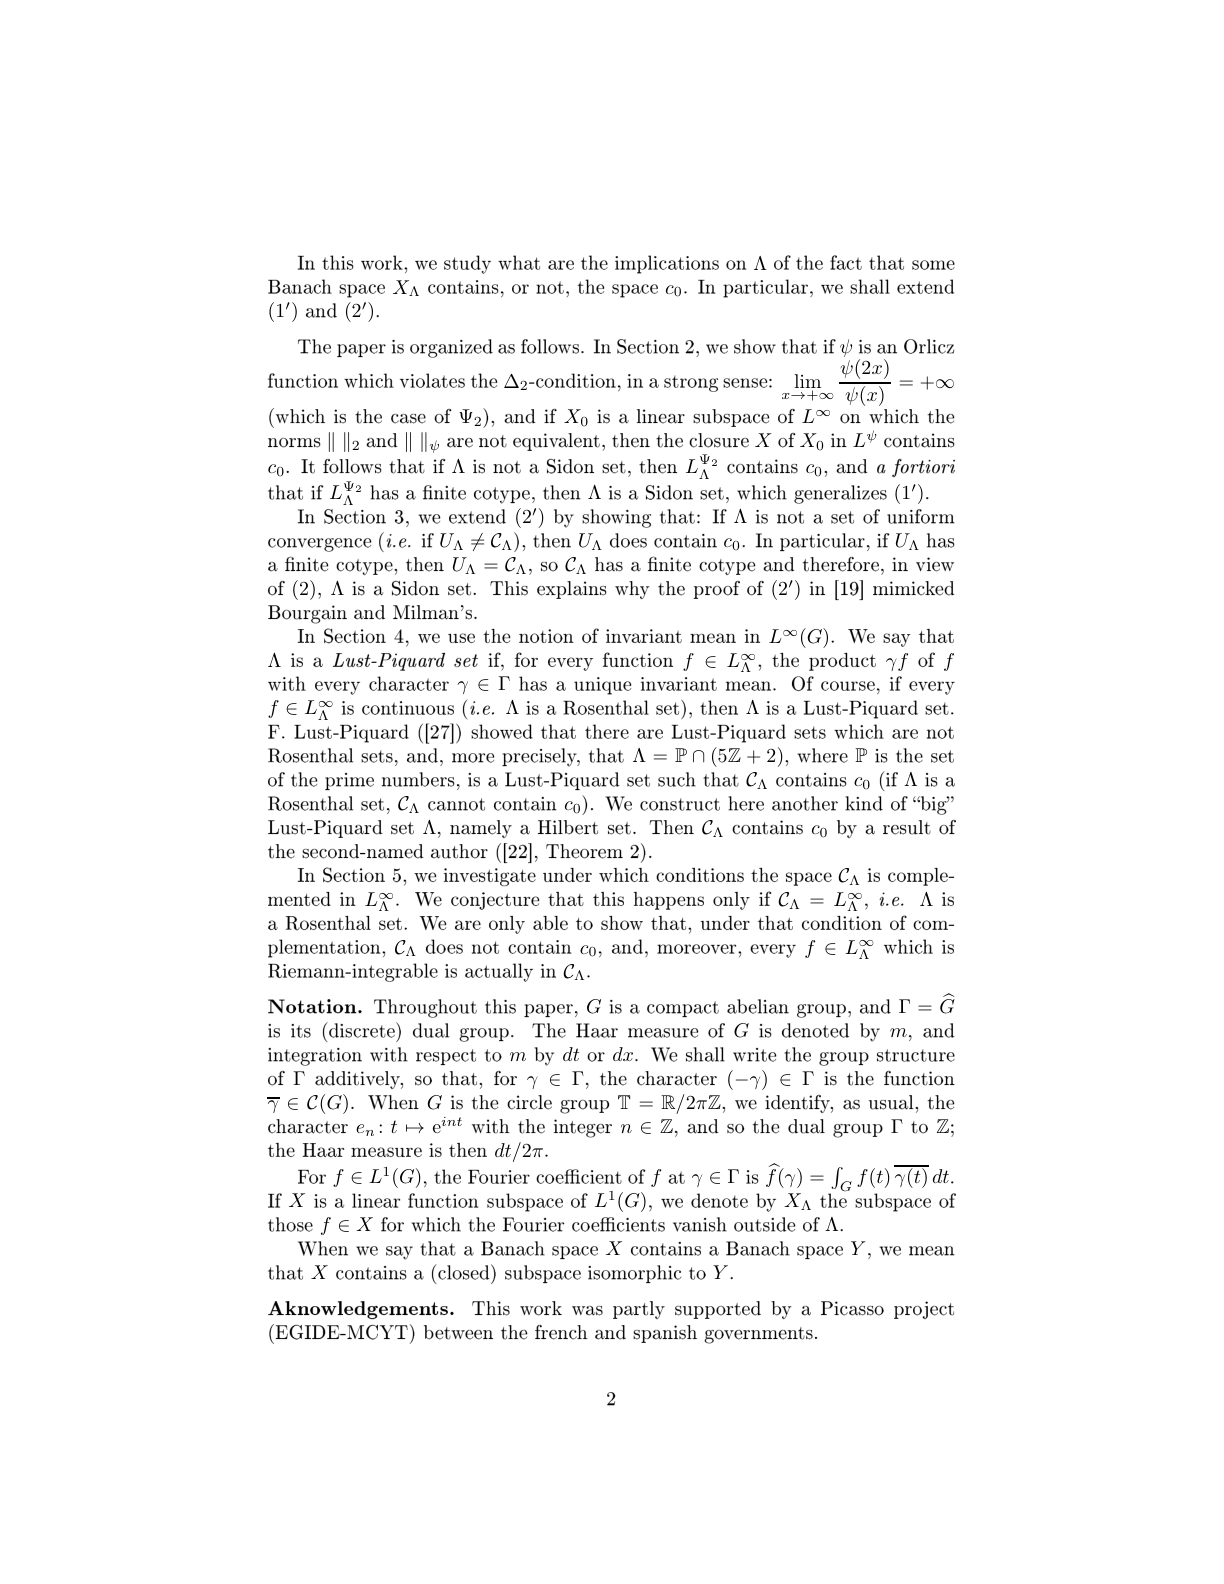
\includegraphics[width=0.88\linewidth]{figures/conjecture_intro_page2.png}
\end{center}

In Section 5 the authors ask whether the existence of a projection from
\(L^\infty_\Lambda\) onto \(\Ccal_\Lambda\) implies that \(\Lambda\) is a
Rosenthal set, and note that they cannot answer this even for norm-one
projections.

\begin{center}
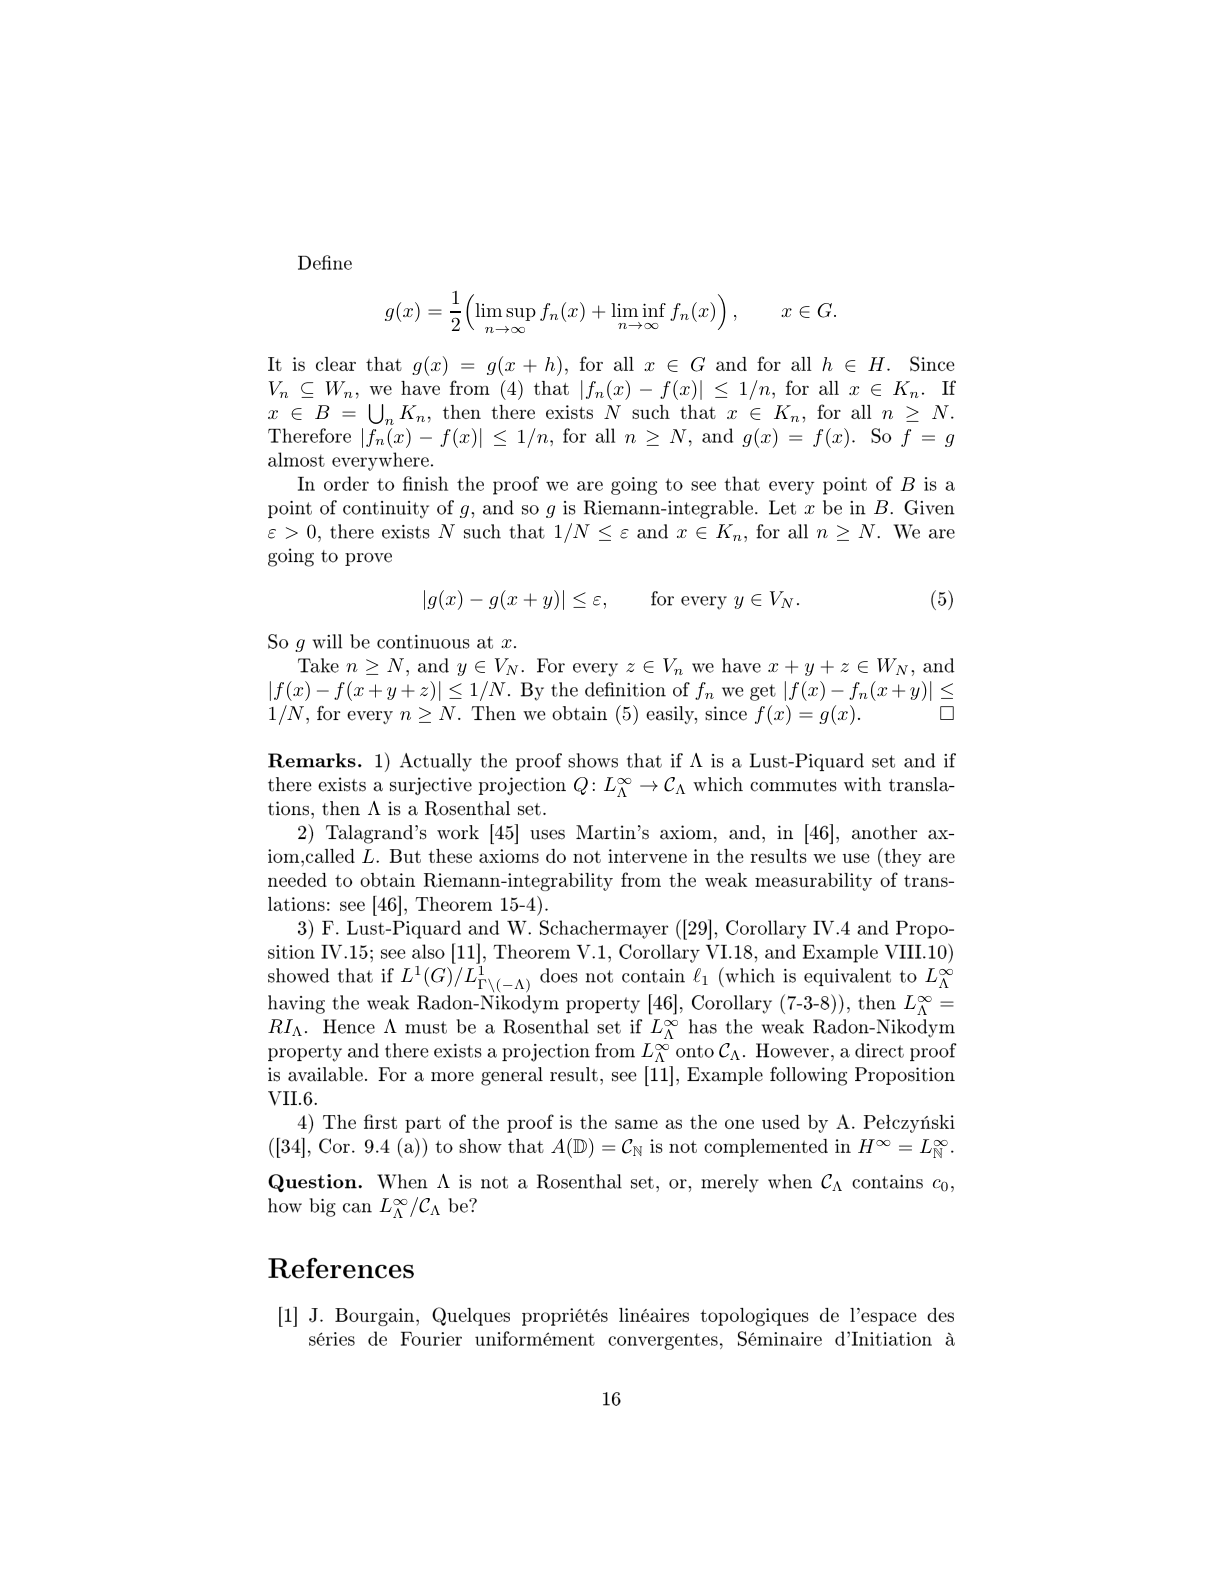
\includegraphics[width=0.88\linewidth]{figures/section5_question_page16.png}
\end{center}

\section*{Definitions}

Let \(G\) be a compact abelian group and let \(\Gamma=\widehat G\) be its
discrete dual group. For \(\Lambda\subseteq\Gamma\), write
\[
L^\infty_\Lambda
=\{f\in L^\infty(G):\widehat f(\gamma)=0\text{ for }\gamma\notin\Lambda\}
\]
and
\[
\Ccal_\Lambda=\Ccal(G)\cap L^\infty_\Lambda .
\]
The set \(\Lambda\) is a Rosenthal set when \(L^\infty_\Lambda=\Ccal_\Lambda\).

\section*{Idea of the Proof}

The only extra hypothesis is weak-star continuity. The continuous
trigonometric polynomials with spectrum in \(\Lambda\) are weak-star dense in
\(L^\infty_\Lambda\). A weak-star continuous projection onto
\(\Ccal_\Lambda\) fixes \(\Ccal_\Lambda\), hence fixes those polynomials, and
therefore fixes their weak-star closure. Thus it must be the identity on all of
\(L^\infty_\Lambda\). Since its range is \(\Ccal_\Lambda\), the two spaces are
equal.

\section*{Theorem}

\begin{theorem}
Let \(G\) be a compact abelian group, \(\Gamma=\widehat G\), and
\(\Lambda\subseteq\Gamma\). Suppose there is a bounded projection
\[
P:L^\infty_\Lambda\longrightarrow \Ccal_\Lambda
\]
which is continuous for the weak-star topology induced by the predual
\(L^1(G)\) of \(L^\infty(G)\). Then \(L^\infty_\Lambda=\Ccal_\Lambda\).
Equivalently, \(\Lambda\) is a Rosenthal set.
\end{theorem}

\begin{proof}
Let \(E_\Lambda=\Lin\{\gamma:\gamma\in\Lambda\}\), the trigonometric
polynomials with spectrum in \(\Lambda\). We first recall the standard
duality fact that the weak-star closure of \(E_\Lambda\) in \(L^\infty(G)\) is
exactly \(L^\infty_\Lambda\).

Indeed, the annihilator of \(E_\Lambda\) in \(L^1(G)\) is
\[
E_\Lambda^\perp
=\{h\in L^1(G): \int_G \gamma h\,dm=0\text{ for every }\gamma\in\Lambda\}.
\]
Taking the annihilator again in \(L^\infty(G)\) gives precisely the functions
whose Fourier coefficients vanish outside \(\Lambda\), i.e.
\((E_\Lambda^\perp)^\perp=L^\infty_\Lambda\). By the bipolar/annihilator
description of weak-star closure, \(E_\Lambda\) is weak-star dense in
\(L^\infty_\Lambda\).

Now let \(f\in L^\infty_\Lambda\). Choose a net \((p_i)\) in \(E_\Lambda\)
which converges to \(f\) in the weak-star topology. Since
\(E_\Lambda\subseteq \Ccal_\Lambda\) and \(P\) is a projection onto
\(\Ccal_\Lambda\), we have \(Pp_i=p_i\) for every \(i\). Weak-star continuity
of \(P\) gives
\[
P f=\text{w}^*\!-\!\lim_i Pp_i
    =\text{w}^*\!-\!\lim_i p_i
    =f .
\]
But \(P f\in \Ccal_\Lambda\), so \(f\in \Ccal_\Lambda\). Since \(f\) was
arbitrary, \(L^\infty_\Lambda\subseteq \Ccal_\Lambda\), while the reverse
inclusion is automatic. Hence \(L^\infty_\Lambda=\Ccal_\Lambda\).
\end{proof}

\section*{Verification and Limitations}

The proof uses only the canonical duality \(L^\infty(G)=L^1(G)^*\) and the
definition of spectral subspaces. It works for arbitrary compact abelian
groups, with no metrizability assumption, because weak-star density is stated
using nets.

This is not a full solution of the source conjecture. The source asks about
arbitrary bounded projections, and explicitly mentions that even norm-one
projections are open. A bounded projection onto a norm-closed subspace of a
dual space need not be weak-star continuous, so the theorem handles only the
normal/weak-star-continuous subcase.

\section*{Novelty Check}

Local index searches for arXiv:0912.3133, \(\Ccal_\Lambda\),
\(L^\infty_\Lambda\), Rosenthal sets, complemented subspaces, and projection
terms found no prior packet. Web searches on 2026-06-16 for the exact
projection/Rosenthal phrases found the source paper but no later exact answer.
The result is a direct subcase proof rather than a literature identification.

\section*{References}

\begin{thebibliography}{9}
\bibitem{LLQR}
P. Lefevre, D. Li, H. Queffelec, and L. Rodriguez-Piazza,
\emph{Some translation-invariant Banach function spaces which contain \(c_0\)},
arXiv:0912.3133.
\end{thebibliography}

\end{document}
